%% ====== Classe du document ============================================
\documentclass[10pt,a4paper]{article}
%\usepackage[left=1.5cm,right=1.5cm,top=2cm,bottom=2cm]{geometry}

%% ====== Francisation ==================================================
\usepackage[french]{babel}
\usepackage[T1]{fontenc}
\usepackage[utf8]{inputenc}
\usepackage{textcomp}

%% ====== Personnalisation ============================================
\usepackage{fancyhdr}
	\lhead{}
	\chead{Projet MDMA - Rapport L2}
	\rhead{M1 IF 2012-2013}
	\renewcommand{\headrulewidth}{0.3pt}
	\renewcommand{\footrulewidth}{0.3pt}
	\lfoot {}
	\cfoot {- \thepage -}
	\rfoot {}
	\pagestyle{fancy}
\title{Projet MDMA - Rapport L2}
\author{}
\date{}

\usepackage{hyperref}

%% ====== Packages pour le texte ========================================
%\usepackage{soul}
%\usepackage[normalem]{ulem}
%\usepackage{fancybox}
%\usepackage{moreverb}
%\usepackage[table]{xcolor}
%% ====== Packages pour les dessins =====================================
\usepackage{float}
\usepackage{graphicx}
%\usepackage{multicol}
%\usepackage{multirow}
%\usepackage{tikz}
%\usepackage{lmodern}
\usepackage{pict2e}

%% ====== Packages pour les maths =======================================
%\usepackage{amsmath}
%\usepackage{amssymb}
%\usepackage{mathrsfs}
%\usepackage{bussproofs}
%\usepackage[ruled,vlined,french]{algorithm2e}

%%% francisation des algorithmes

%\usepackage[squaren,Gray]{SIunits}
%% ====== Reglages generaux =============================================

\usepackage{titlesec}
	\titleformat{\section}[frame]
	{\normalfont}
	{\filright
	\footnotesize
	\enspace Partie \thesection\enspace}
	{6pt}
	{\bfseries\filcenter}
	
	\titleformat{\subsection}[frame]
	{\normalfont}
	{\filright
	\footnotesize
	\enspace \thesubsection\enspace}
	{6pt}
	{\filcenter}
%	{\titlerule
%	\vspace{.8ex}%
%	\normalfont\itshape}
%	{\thesubsection.}{.5em}{}

	\titleformat{\subsubsection}
	{\titlerule
	\vspace{.8ex}%
	\normalfont\itshape}
	{}{.5em}{}

\titleformat{\chapter}[display]
	{\normalfont\bfseries\filcenter}
	{}
	{1ex}
	{\titlerule[2pt]
	\vspace{2ex}%
	\LARGE}
	[\vspace{1ex}%
	{\titlerule[2pt]}]
	
\parindent=10pt

%\usepackage{makeidx}
%\makeindex
%\newcommand\vect{\overrightarrow}

%\numberwithin{equation}{subsection}


\graphicspath{{img/}}


%% ================================================================
\begin{document}
\maketitle
\newpage

\tableofcontents
\newpage
%% ================================================================
\section{Design Interface}
\subsection{Participants}
\begin{itemize}
    \item Hadrien Croubois (responsable d'équipe);
    \item Luc Rocher
\end{itemize}
\subsection{Objectifs}
\par Le \emph{workpackage} "Design Interface" a pour objectif de mettre au point et d'implémenter l'interface ainsi que de penser a l’interconnexion de l'interface avec l'ensemble des composants du logiciel. Il s'occupe en plus de la gestion des configurations décrites par l'utilisateur, qu'il s'agisse de leurs paramétrages via les différentes fenêtres ou de la partie chargement/enregistrement. La connaissance de l'état d'avancement des différents \emph{workpackages} permet de définir efficacement les formats de configuration ainsi que de penser les flux de données nécessaires a l'affichage au cœur de la structure du programme.
\par Le \emph{workpackage} "Design Interface" anticipe a ce titre une part de l’intégration.
\subsection{Avancement}
\par L'interface en elle même est écrite a l'aide du designer de fenêtre de \emph{QtCreator}\footnote{QtCreator - \url{http://doc.qt.digia.com/qtcreator/index.html}}.
\par La fenetre principale permet, en plus de la visualisation de l'image acquis par la webcam de charger et sauvegarder differentes configuration ainsi que d'avoir un resumé des differentes zones definies. Ces zones peuvent être crées en cliquant sur la video, modifiées et supprimées.
\begin{figure}
    \centering
    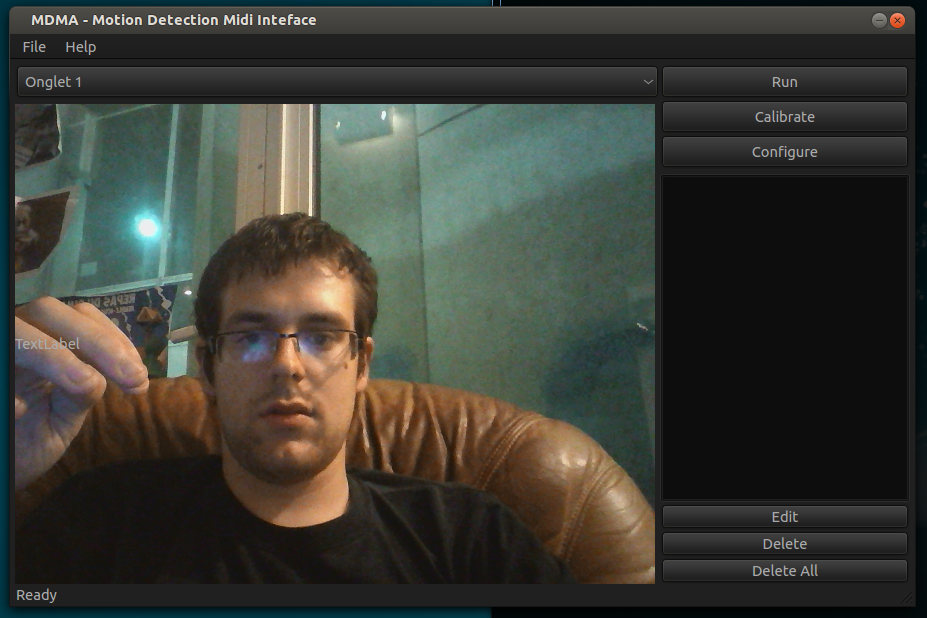
\includegraphics[width=12cm]{design_window.png}
    \caption{La fenêtre principale de l'interface}
\end{figure}
\par L'ouverture d'une nouvelle configuration ou la fermeture du programme alors que la configuration actuelle a ete récement modifiée demande a l'utilisateur de sauvegarder la configuration actuelle.
\par Un bouton "Calibrate" lancera une procédure de calibration, de meme que le bouton "Configure" ouvre une fenetre permettant de choisir différentes options (caméra si plusieurs sont disponible, port midi ...).
\par Un bouton Run lance le programme. Une fois lancé, la configuration n'est plus éditable (les differents boutons sont desactivés). Seul le bouton "Run", renommé en "Stop", reste actif et permet d'arrêter le programme.

\section{OpenCV Interface}
\subsection{Introduction}
\par Le tâche prise en charge initialement par les contributeurs du workpackage consistait en la création du module qui capturerait l'image de la camera, localiserait les mains sur cette image et transmettrait la totalité des informations : la position des mains, leur vitesse, leur accélération et la forme (fermée ou ouverte). La spécification initiale du système sous-entendait la possibilité que le système fonctionne sans utiliser de matériel onéreux.
\subsection{Conditions de fonctionnement}
\par Pendant le développement, il était entendu que la reconnaissance des mains se ferait sans avoir recours à des marqueurs et sans l'utilisation de matériel spécial (comme par exemple l'outil Microsoft Kinect). Après avoir considéré certaines contraintes pour assurer la reconnaissance des mains, l'équipe de ce workpackage a décidé d'utiliser des gants noirs. Les tests ont montré que la reconnaissance des mains avec les gants est stable sous les quelques conditions suivantes : 
\begin{itemize}
\item Le fond ne contient pas d'objets foncés.
\item Le vêtement d'utilisateur est notablement plus clair que les gants, qui doivent être très foncés (noirs).
\item L'éclairage doit être suffisant. 
\end{itemize}
\par Du point de vue logiciel, le module nécessite que la librairie OpenCV soit installée sur le système. 
\par Comme extension du projet, nous envisageons de développer une version de notre logiciel fonctionnant avec une Kinect. La version ne sera qu'optionnelle tant qu'elle demandera les dépenses supplémentaires de part de l'utilisateur. Malgré ce défaut le développement de la version est bien raisonnable tant qu'il assure la reconnaissance grâce à l'utilisation des matériels dont la prédestination est le tracking des objets. 
\subsection{Algorithme développé}
\par Vers ce moment le résultat est l'algorithme développé et implémenté avec l'utilisation de librairie OpenCV. L'implémentation développée d'une manière qui lui permet d'être plate-forme-indépendante.
\subsubsection{Structure de l'algorithme}
\begin{itemize}
\item Calibration du système. L'utilisateur place les mains dans les zones spéciales. Après cela le système fixe $L'$ égal éclairage du point le moins éclairé dehors de ces zones. $L=L'-\Delta$ devient le seuil critique de luminosité. Après cette étape le main boucle infini du fonctionnement se déroule.
\item Commencement du boucle. Capture de l'image.
\item Conversion RGB $\to$ Grayscale. 
\item Création du masque. Les 1 prennent place de tous les pixels dont la luminosité est moins que $L$.
\item Masquage des pixels de la zone morte dédié pour le corps de l'utilisateur. Les pixels de la zone se rendent égaux 0.
\item L'érosion de l'image. 
\par Définition de l'érosion. L'érosion est l'une des deux opérations fondamentales du traitement d'image morphologique. Soit A une image binaire et B un élément de structure. L'érosion de A par B est donné par : $A \bigodot B = \{z|(B)_z \subset A\}$.
\par Pour l'élément structurant dans l'implémentation nous utilisons ellipse $3 \times 3$.
\begin{table}[h]
\centering
\begin{tabular}{|c|c|c|}
\hline
0 & 1 & 0 \\ \hline
1 & 1 & 1 \\ \hline
0 & 1 & 0 \\ \hline
\end{tabular}
\caption{Élément structurant: ellipse $3 \times 3$}
\end{table}
\par L'érosion est utilisée pour la filtration du bruit: petites particules blanches qui peuvent apparaître sur le masque par hasard. L'érosion est appliquée au masque 2 fois.
\item La dilatation de l'image.
\par La dilatation a pour le but compenser l'utilisation de l'érosion et simplifier les frontières des objets. La dilatation est définie comme $A \bigoplus B = \cup_{b \in B}A_b$. Pour la dilatation le même élément structurant que pour l'érosion dans l'étape précédente. 
\item La recherche des contours. La recherche des contours est faite avec l'utilisation de l'algorithme de Teh-Chin \footnote{Teh, C.H. and Chin, R.T., On the Detection of Dominant Points on Digital Curve. PAMI 11 8, pp 859-872 (1989)}.
\item La construction de l'enveloppe convexe. Les points des contours sont divisés en deux ensembles selon la partie de l'image (gauche ou droite) à laquelle ils appartiennent. Pour chaque ensemble on construit une enveloppe convexe avec l'algorithme de Sklansky \footnote{Sklansky, J., Finding the Convex Hull of a Simple Polygon. pp 79-83 (1982)
}.
\item Le moyen des coordonnées de chaque enveloppe est considéré comme la coordonnée de la main. Gardant l'histoire des positions des mains on peut calculer la vitesse et l’accélération. 
\item On recommence la boucle.
\end{itemize}
\subsection{Roadmap}
\par Comme l'algorithme est développé et testé il ne reste que l'intégration avec workpackage Gestion des événements. C'est à dire il reste créer l'objet actif qui offre l'interface au module de gestion des événements. 
%% Caractérisation des événements
%% ---------------------------------------------------
\section{Caractérisation des événements}
\subsection{Introduction}
\par Le workpackage de caractérisation des évènements se charge du déclenchement des signaux MIDI fournis par l'interface MIDI lorsque des évènements sont détectés dans des zones décrites par l'utilisateur et de l'affichage en surimpression des zones activées. Les spécifications nous donnent les types d'évènements qu'il faut pouvoir détecter et quels types de zones on doit disposer et l'interface MIDI nous fournit ce qu'on doit envoyer. Il s'agit donc d'implémenter la détection d'évènement, le déclenchement des signaux et le dessins des zones.
\subsection{Description des zones}
\par Une zones est décrites initialement par sa position, sa taille, son type (fadder, pad ou segment) et, pour chaque évènement, un ensemble de signaux MIDI (éventuellement vide) qui doivent être déclenché lorsque cette évènement est détecté. Les évènements que l'on souhaite repéré dans une zone sont l'ouverture et fermeture de main, le déplacement de main, le franchissement pour un segment et l'entrée et la sortie pour un pad. (les pads XY seront gérés comme des fadders à axes doubles)
\par Pour détecter un évènement, on dispose de deux positions de la main, l'actuelle et la précédente et de l'état de la main, ouverte ou fermée. De ces informations on détecte directement l'entrée/sortie d'une zone, le franchissement d'un segment. Pour les autres évènements, il nous faut également l'état de la zone :
\begin{itemize}
    \item active ou non pour lancer ou arrêter un clip
    \item l'ouverture de la main à l'entrée dans la zone pour les fadders, une main qui rentre fermée dans un fadder ne doit pas changer sa valeur.
\end{itemize}
\par Une fois un évènement détecté, on envoie les signaux correspondant à l'interface midi.
\subsection{Implémentation}
\par La détection ET le déclenchement de signaux sont réalisés par les zones. La gestion des évènements consiste à envoyer à chaque zone/segment les informations suffisantes relatives à la main. Il s'agit donc d'une boucle disposant de la liste des zones (fournis par la configuration) qui la parcourt en appelant pour chaque zone la détection.
\subsection{Affichage des zones}
\par Cette partie n'a pas encore été codé car est le résultat de notre dernière réunion. Les zones et les segments seront dessinés sur un Label Qt puis sera superposé à l'image de la caméra avec de la transparence. Il s'agit de montrer quelles zones sont actives et donc d'offrir un support visuel à l'utilisateur. 

\section{\emph{Workpackage} Communication}
\subsection{Introduction}
\par Le \emph{workpackage} «~communication~» est composé de trois personnes : Luc Rocher (responsable d'équipe), Timothée Bernard \& Hadrien Croubois.
\par Il s'occupe de la communication du projet sur deux échelles, en externe et en interne. La communication externe concerne l'ensemble des liens entre \emph{MDMA} et les acteurs extérieurs (que ce soit par voie numérique -- site Web, courriels -- ou par voie orale). La communication interne est chargée de gérer les discussions dans l'équipe, ainsi qu'avec les responsables du projet et du département.
\subsection{Définition d'une identité graphique}
\par Pour débuter une bonne communication, il faut d'abord réfléchir à l'image que l'on veut donner au projet. MDMA a pour but de développer un logiciel innovant : l'interface homme-machine se veut délibérément moderne, sans clavier ni souris l'utilisateur peut commander son ordinateur pour produire des signaux musicaux. Mais il s'inscrit dans une tendance alternative, celle de la musique électronique et des synthétiseurs sonores. Nous avons cherché à construire une identité assez \emph{rétro} mais véhiculant la nouvauté du projet.
\par Nous sommes parti d'un ensemble de couleurs très vivantes -- du jaune au rouge -- assez agressives :
\begin{figure}[H]
  \centering
  
\includegraphics[width=10cm]{comm-swatch.pdf}
  \caption{Gamme de couleurs utilisées pour la charte graphique}
  \label{fig:swatch}
\end{figure}
\par Avec ces couleurs, nous avons pu réfléchir à un logotype. Plusieurs pistes étant possible, celle d'un texte uniquement (« MDMA ») assez minimaliste a été privilégié, avec une police très \emph{pixelisée}. Trois propositions ont été réalisées pour affiner le logo :
\begin{figure}[H]
  \centering
    
\includegraphics[width=8cm]{comm-logos.pdf}
  \caption{Trois propositions de logotype}
  \label{fig:Logos-MDMA}
\end{figure}
\par Le premier graphique a été sélectionné par l'équipe, et rapidement intégré au site Internet.
\subsection{Communication numérique}
\subsubsection{Site Internet}
\par Afin d'obtenir un minimum de visibilité, le projet avait besoin d'une présence sur Internet. Nous avons donc d'abord travaillé à mettre en place un site Web. Nous avons travaillé sur une interface assez minimaliste, fondée sur les couleurs de la gamme représentée à la figure~\ref{fig:swatch}.
\par Le site Internet (\url{http://graal.ens-lyon.fr/mdma/}) contient différentes informations, dont :
\begin{itemize}
  \item une présentation du projet, minimale sur la première page, puis détaillée par la suite ;
  \item une description complète de chaque \emph{workpackage} ainsi que leurs avancées et découvertes au fil du temps ;
  \item une page personnelle pour chaque membre, avec la possibilité de nous contacter.
\end{itemize}
\par Le site est fondé sur Wordpress -- un moteur dynamique -- qui nous permet de gérer des commentaires pour chaque page, une première page dynamique avec la liste des derniers articles, des flux RSS… Par ailleurs, un \textbf{travail de traduction} a été réalisé sur presque l'intégralité du site, pour obtenir un site entièrement bilingue, en français et en anglais. Un menu en haut du site contient des boutons avec icônes pour sélectionner la langue ; par ailleurs, selon la langue du navigateur, la langue optimale est automatiquement choisie.
\begin{figure}[H]
  \centering
    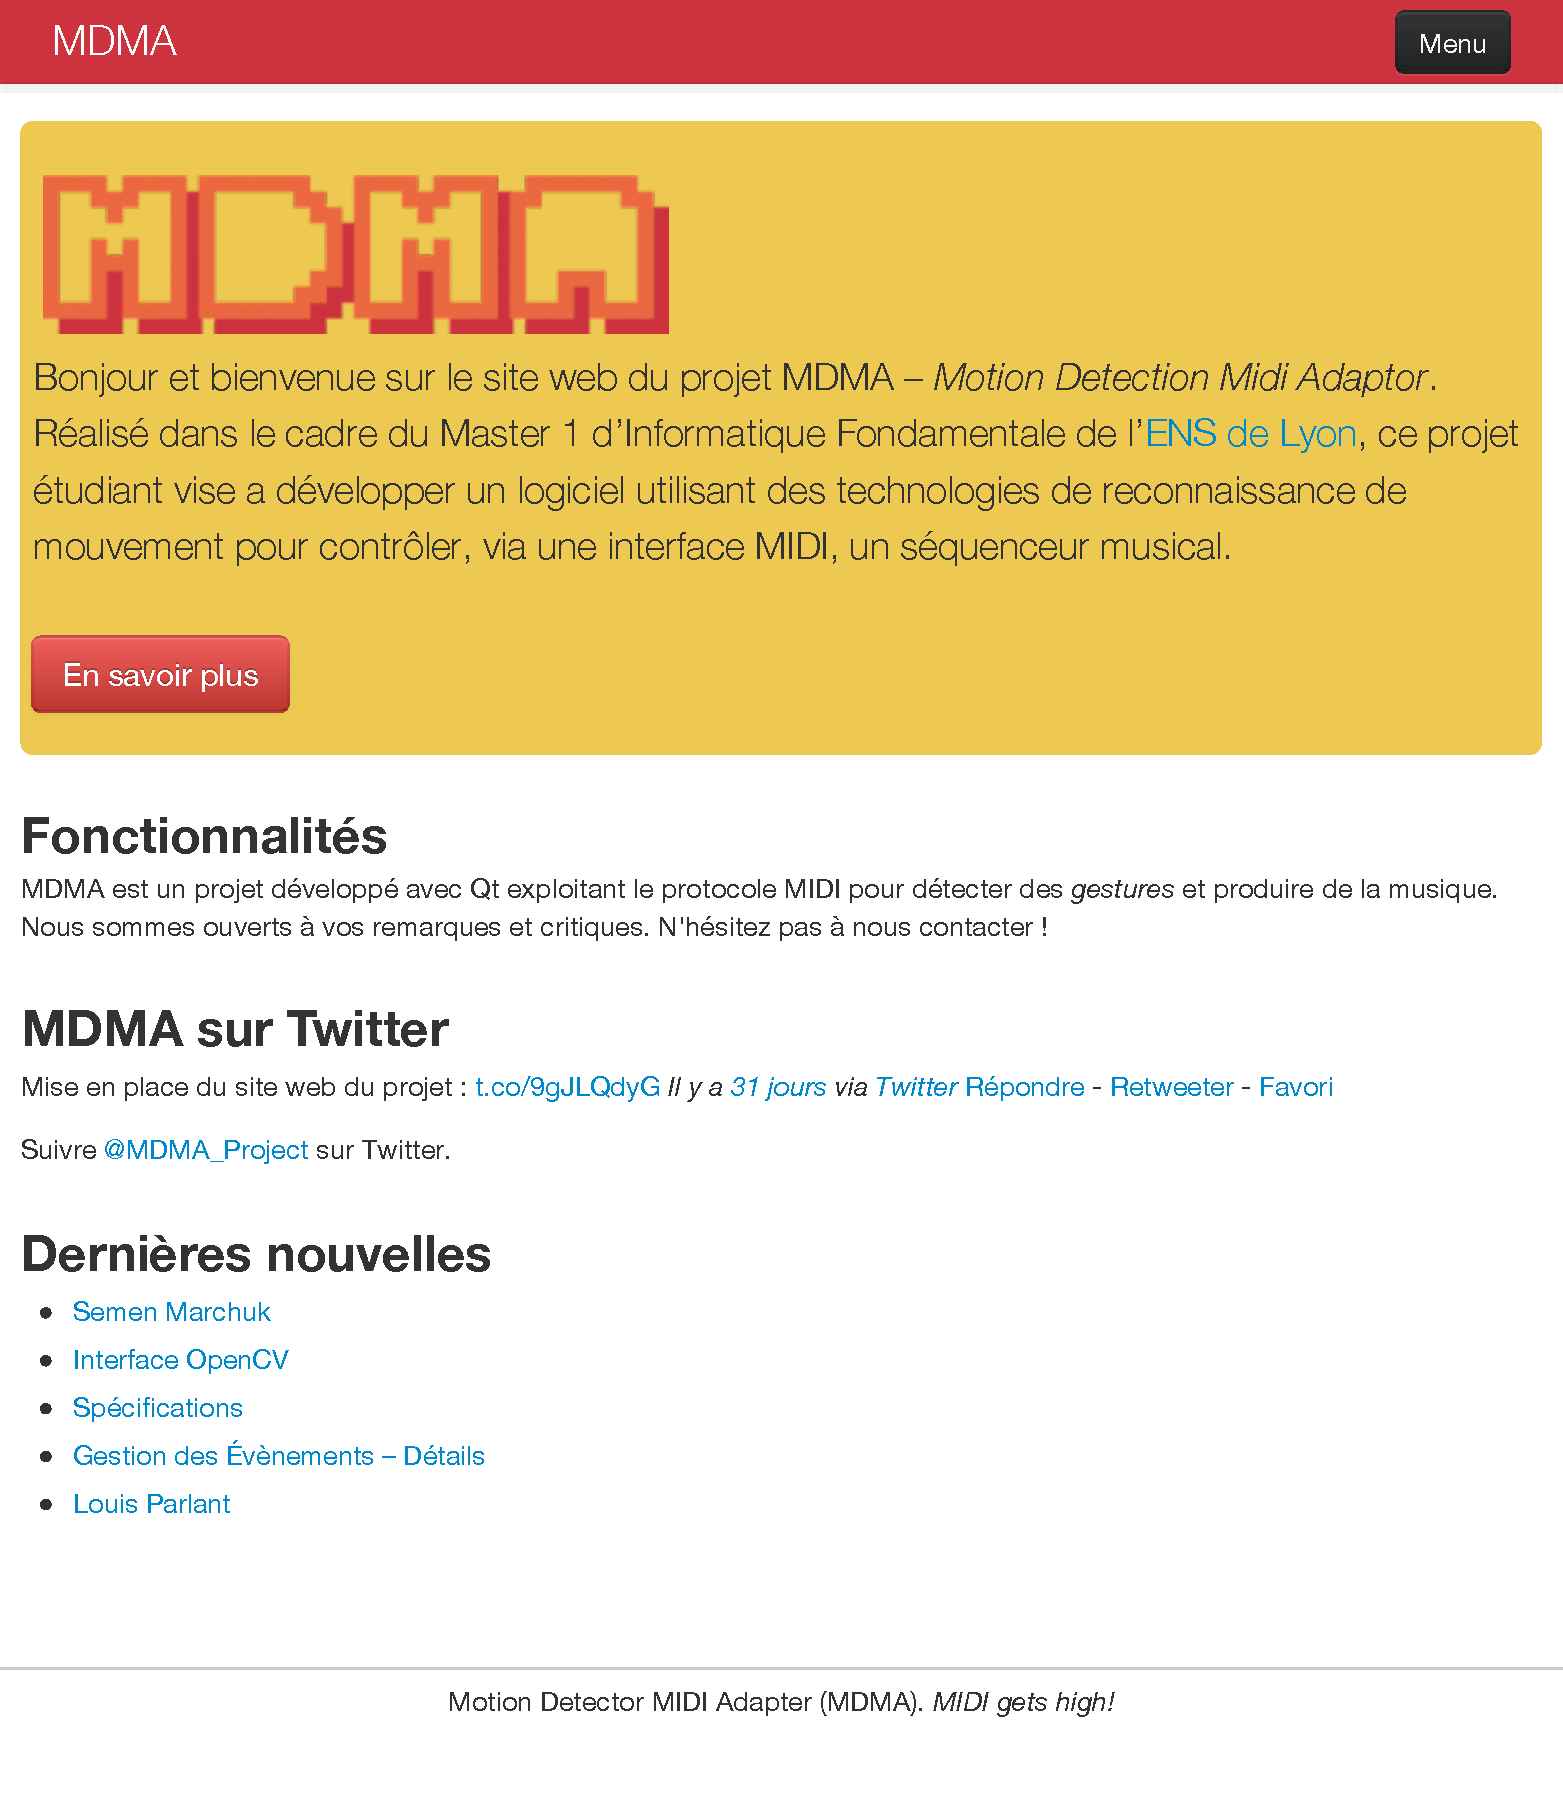
\includegraphics[width=8cm]{comm-web2.pdf}
  \caption{Capture d'écran du site (version mobile)}
\end{figure}
\begin{figure}[H]
  \centering
    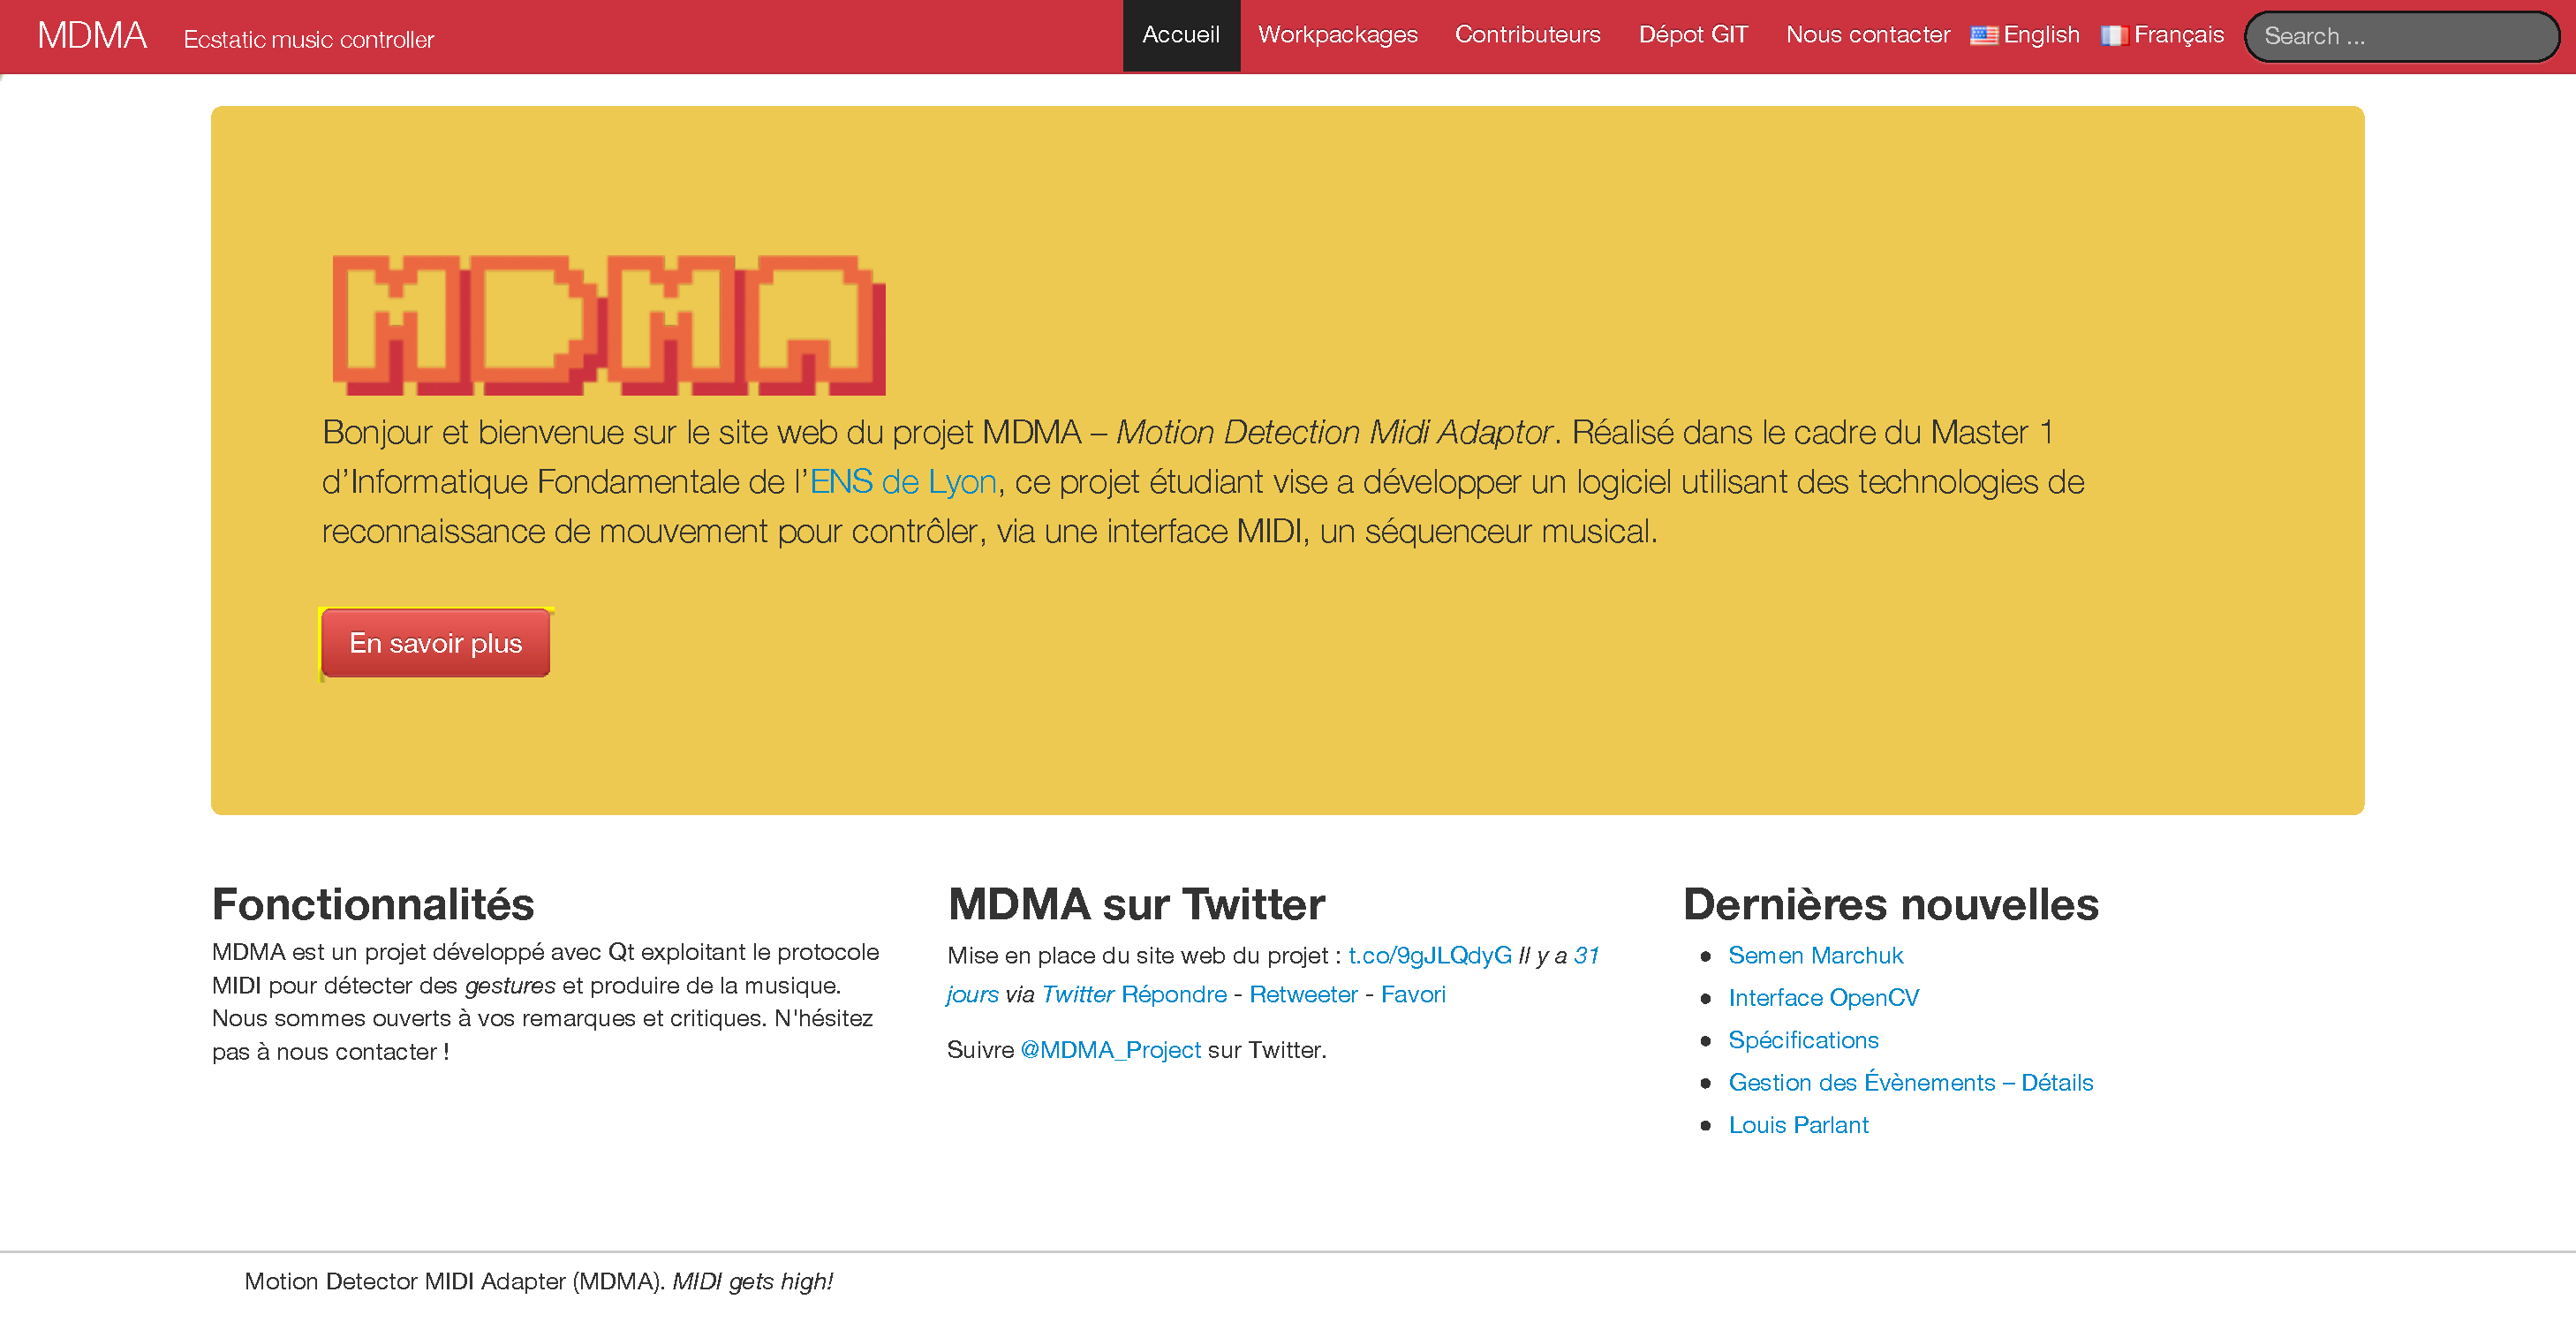
\includegraphics[width=10cm]{comm-web1.pdf}
  \caption{Capture d'écran du site du projet}
\end{figure}
\subsubsection{Autre présence}
\par Le projet dispose aussi d'un page sur Facebook (\url{http://www.facebook.com/mdma.project}) et d'un compte Twitter. Ces espaces ne sont pas très actifs, mais pourront le devenir dès que le projet disposera d'un logiciel fonctionnel et pouvant être diffusé.
\subsection{Diffusion numérique}
\par L'équipe « communication » se charge du lien entre le projet et l'équipe pédagogique, par exemple pour des questions de budget (le financement récent d'un Microsoft Kinect par exemple) ; il a aussi pour vocation de diffuser notre projet à des musiciens et des personnes intéressées par la musique électronique. Nous chercherons ainsi des utilisateurs capable de tester MDMA et de produire des retours en situation réelle. Cette axe là pourra se développer dans les semaines qui viennent, avec la finalisation du logiciel.
\subsection{Bilan}
\par À l'orée de la moitié du projet, la communication a réalisé une grande partie du travail nécessaire. Il reste encore à rajouter du contenu sur le site, à favoriser les échanges avec les professionnels de la musique, et pourquoi pas à étudier un volet \emph{presse}.

%% ===================================================================
\end{document}
